\chapter{Experiments}
\label{chapter:experiments}

In this chapter, we will look at the configuration of the experiments, which has a direct impact on the results of our four different approaches to anomaly detection. Before running the experiments, we will also look at the data visually to verify the accuracy of the assumptions we make about the data. We then present the experimental setup, including the datasets, the software and hardware used for the experiments, and the evaluation metrics. Finally, we present the definitions of the tunable hyperparameters and give an overview of the hyperparameter values that performed best and will be used for the final experiments.

\section{Exploration of Assumptions}
To gain better insight into the dataset, it is useful to perform an initial Exploratory Data Analysis (EDA) \cite{eda} of our dataset. Exploratory data analysis is used to analyze the underlying structure of the data and summarize the main features, often via visualization methods. Visualization helps us to test our assumptions and formulate hypotheses about the data, which are important to choose the right approaches and parameters for anomaly detection. In addition, visualization of the logs helps us answer \textbf{RQ1} (Research Question 1).

For visualization, we use the numerical representation of our dataset obtained by feature extraction. All visualizations in the following sections were obtained on the event count embedding of the data. The embedding of the log sequences contains \featureVectorLength\ variables. Data with such high dimensions are difficult to interpret. Therefore, it is necessary to use dimensionality reduction techniques. To perform initial exploration as well as visualize the anomaly detection results, we will use two algorithms, PCA and t-SNE, to reduce the dimensionality for data visualization:

\begin{itemize} 

\item \textbf{Principal Component Analysis (PCA)} \\ One way to reduce the dimensionality of data without losing too much information is to use Principal Component Analysis (PCA) as an unsupervised tool for exploratory data analysis. In PCA, the data points (in our case, the feature vectors) in our\\ \featureVectorLength-dimensional feature space are transformed to a 2-dimensional feature subspace. Moreover, the variables in the new artificial subspace (principal components) are not correlated. The first principal component (PC1) propagates in the x-axis direction and explains most of the variance in the data.
    
   \item \textbf{t-distributed Stochastic Neighbor Embedding (t-SNE)}\\ t-SNE is a recent algorithm for dimensionality reduction into a two or three dimensional space that is particularly well suited for data visualization \cite{tsne}. PCA is a linear method that keeps the dissimilar data points far apart in the low-dimensional projection. In contrast to PCA, t-SNE is a non-linear method. It focuses on preserving the local structure by keeping the high-dimensional data points that lie on or near a nonlinear manifold in the lower dimensions close together. Preserving local structure while revealing important global structure is the main advantage over linear techniques, where this is usually not possible.
    
\end{itemize}

The four assumptions we will explore with respect to the collected data are the following: 

\begin{itemize} 
    \item \textbf{Assumption 1:} Daily dataset deviates too much from the normal behaviour represented by Nightly to be used for training purposes 
    \item \textbf{Assumption 2:} Using data from nightly tests collected in a single night for training is sufficient because the data from all nightly tests are equivalent 
    \item \textbf{Assumption 3:} Logs generated from calls between two radios are\\
    grouped into a call cluster when plotted 
    \item \textbf{Assumption 4:} Different anomaly logs are grouped into distinct and clearly separated clusters when plotted
\end{itemize}

We will describe each assumption in detail in the next sections.

\subsection{Choosing Data for Training: Daily vs Nightly}
\label{assumption-daily-vs-nightly}

As we explained in the earlier sections of this chapter, we train the models on the Nightly dataset under the assumption that its data points are normal. On the other hand, we have no prior assumptions about the Daily dataset and about the distributions in it. Therefore, we want to make a simple visual comparison between the Daily and Nightly datasets. Next, we wanted to determine if the Daily data points fall within the normal range.

Figure \ref{fig:tsne-single} shows two visualizations of applying t-SNE to the Daily and Nightly datasets. The t-SNE analysis of the Daily data appears to split the data into four visual clusters. Although it is difficult even for domain experts to interpret what each cluster represents, we assume that the developers tested four different features on the day they obtained the Daily dataset, resulting in the groupings of data points in each cluster.

The visualization of the t-SNE in the plot of the Nightly dataset shows that most of the data points are packed together and form a cluster. However, there is a group of points at the bottom of the plot that appears to be quite distant from the rest of the points and could be considered an outlier. Looking more closely at the raw logs behind the data in this cluster, we found that they contain a high number (about $400$ hundred logs every two minutes) of log messages informing about a call, as shown in the following event templates:

\begin{itemize}
    \item \texttt{\justify Call \{1586,1\} \{:call\_number, <*> <*> forwarding audio RtpPacket\{ssrc: <*> urid: <*> timestamp: <*> seq\_num: <*>}
    \item \texttt{\justify Call \{1586,1\} \{:call\_number, <*> <*> received RtpPacket\{ssrc: <*> urid: <*> timestamp: <*> seq\_num: <*> from \{228, 28, <*> <*>}
    \item \texttt{\justify Call \{1586,1\} \{:call\_number, <*> <*> forward RtpPacket\{ssrc: <*> urid: <*> timestamp: <*> seq\_num: <*> LMR: [ssrc: <*> urid: <*> to \{228, 28, <*> <*>}
\end{itemize}

This is further confirmed by visualizing the Call dataset in respect to the Nightly dataset in Assumption \ref{assumption-calls}.

Since calls are not frequent during testing phase, compared to other processes running in the system, this is exactly what we expect to see reflected in the logs. Nonetheless, as shown in the plot, the cluster is considerably distant from the rest of the points, and we do not want regular calls to be detected as anomalies. It is important to note here that the distances between clusters in t-SNE do not necessarily mean anything. Fine-tuning the \textit{perplexity} hyperparameter of t-SNE is required to obtain clusters that maintain global geometry. Thus, we do not know where the assumed call cluster lies with respect to the rest of the data points.

\begin{figure}%
    \centering
    \subfloat[\centering Nightly Dataset]{{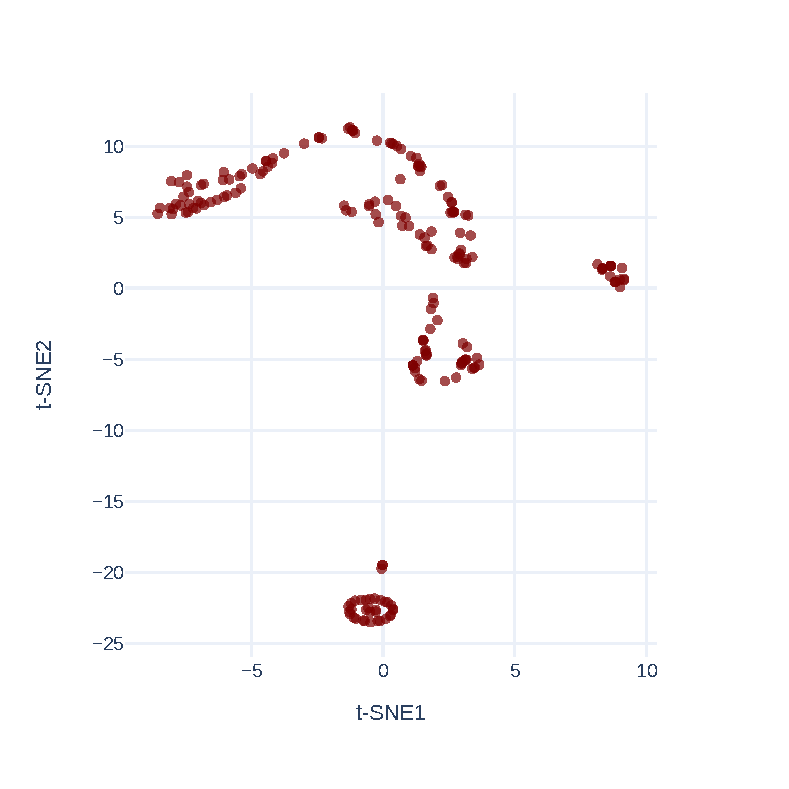
\includegraphics[width=5.52cm]{img/tsne-nightly.pdf}}}%
    \qquad
    \subfloat[\centering Daily Dataset]{{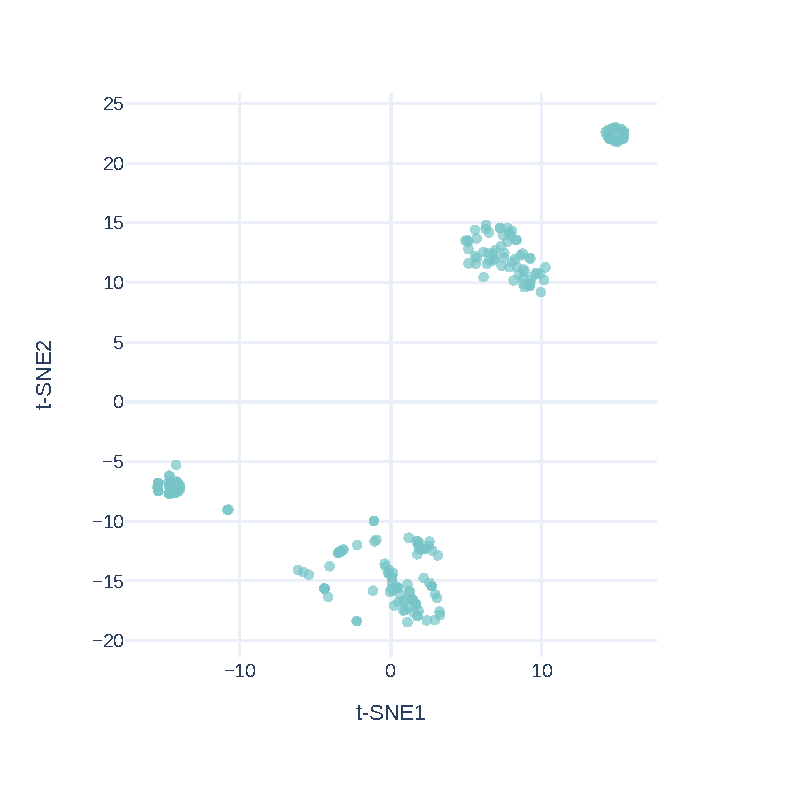
\includegraphics[width=5.52cm]{img/tsne-daily.pdf}}}%
    \caption{Application of t-SNE to the event count vector embeddings of the Nightly and Daily datasets.}%
    \label{fig:tsne-single}%
\end{figure}

Finally, we are interested in seeing how PCA compares to t-SNE, and we also want to plot the Daily and Nightly datasets relative to each other. Figure \ref{fig:pca-nightly-daily} shows a plot of the first two principal components after performing principal component analysis on the Nightly and Daily datasets. Figure \ref{fig:tsne-nightly-daily} is a t-SNE plot visualizing the Nightly and Daily datasets.

The points produced by PCA appear to be much denser compared to t-SNE, but there is very little overlap between the Daily and Nightly data in either plot. One way to explain this is that the tests performed at night do not fully cover the behaviour of the system. Another explanation, confirmed by the developers at Motorola as the most likely, is that the experiments conducted during the day vary each day depending on the feature being tested, and it may also behave completely opposite to what we consider normal behaviour. Nonetheless, these visualizations confirmed that the Daily dataset should not be used for training the models because it is unpredictable and inconsistent. It is still a good candidate for performing expert validation on an unlabeled dataset, where an expert's understanding of the underlying processes will help us understand the anomaly detection models.

\begin{figure}[h]
    \centering
    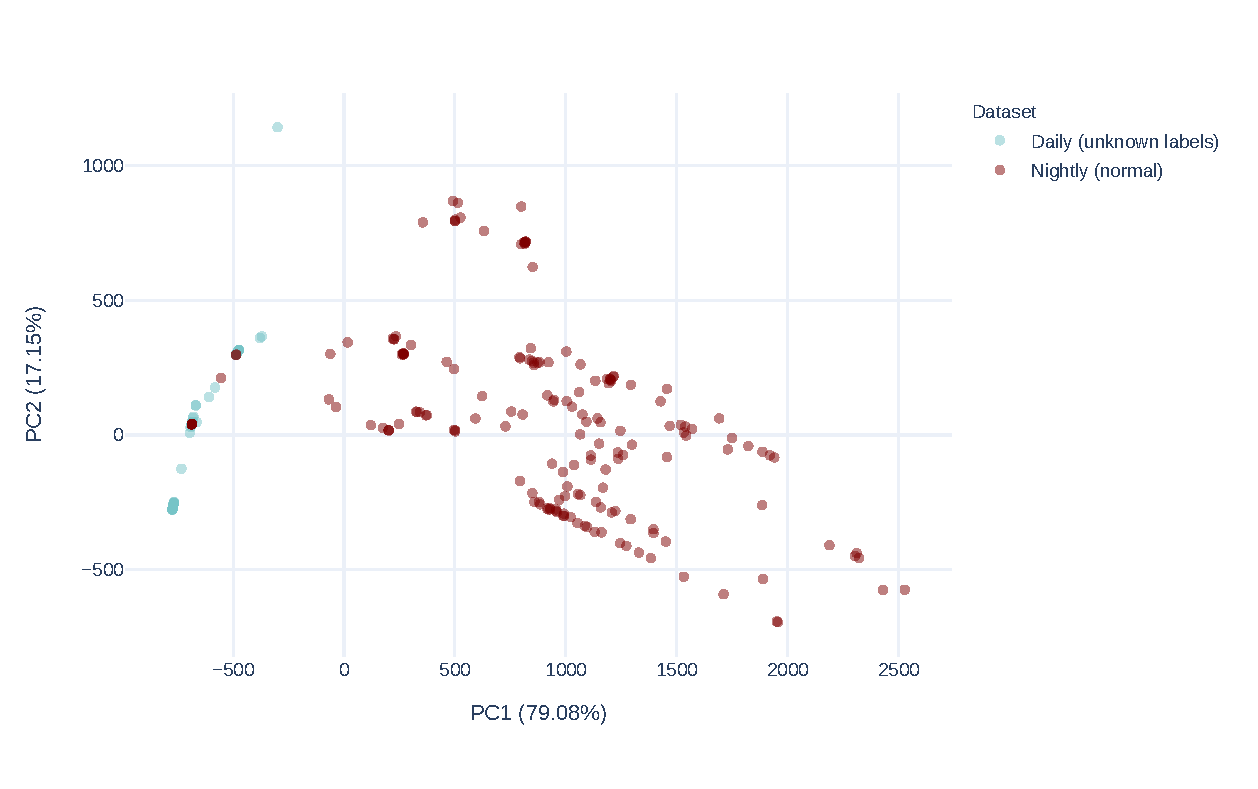
\includegraphics[width=\textwidth]{img/pca-nightly-daily.pdf}
    \caption{Application of PCA to the Daily and Nightly dataset}
    \label{fig:pca-nightly-daily}
\end{figure}

\begin{figure}[h]
    \centering
    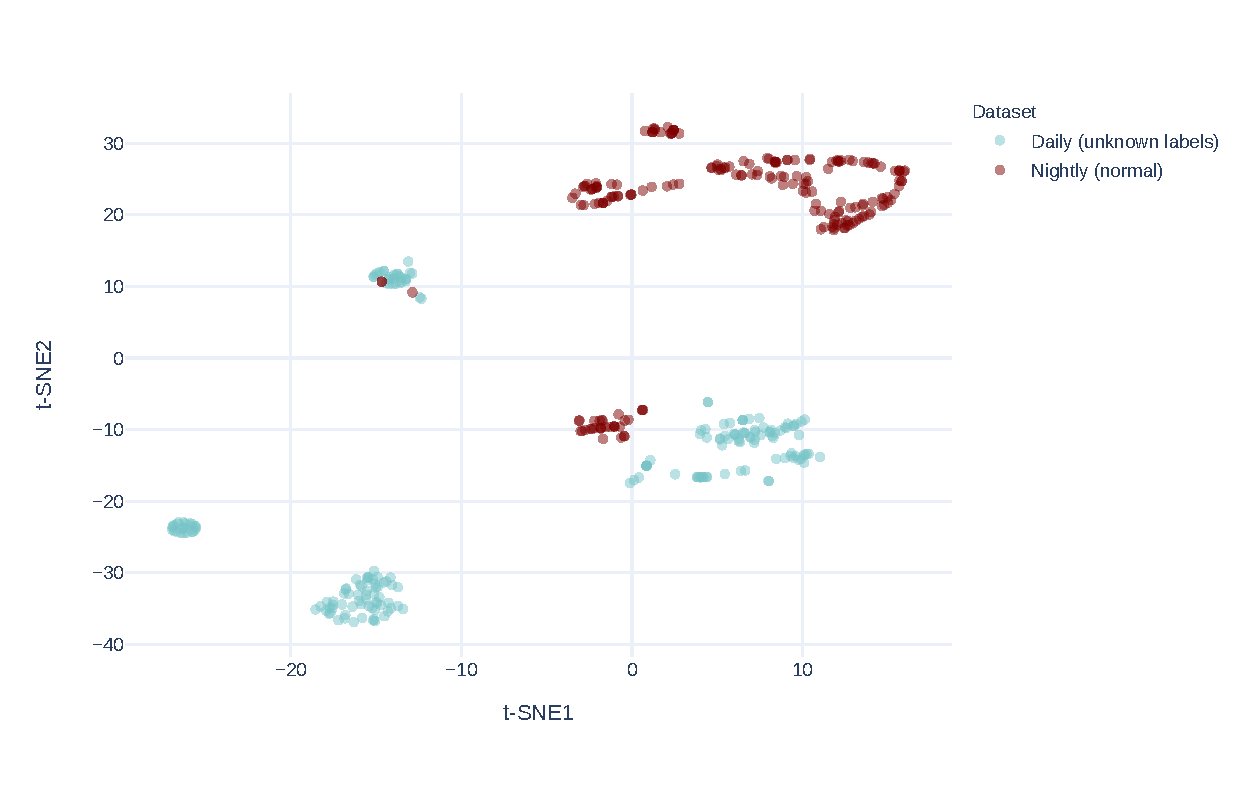
\includegraphics[width=\textwidth]{img/tsne-nightly-daily.pdf}
    \caption{Application of t-SNE to the Daily and Nightly dataset}
    \label{fig:tsne-nightly-daily}
\end{figure}

\subsection{Completeness of the Nightly Dataset}
\label{assumption-completeness}

Another important question we would like to answer by conducting EDA concerns the completeness of the Nightly dataset from January 24, 2021, which we would like to use for training the one-class model: \textit{Do the data from the nightly tests differ across dates?} \textit{Would merging data from multiple nightly test datasets provide additional information about the normal behaviour of the system?}

To analyze the data and answer these questions, we will again use PCA and t-SNE and plot the data from two different nights of testing. Figure \ref{fig:tsne-nights-comparison} shows the visualization of the results. It can be seen that the two data sets overlap almost completely in both the PCA and t-SNE plots. Given the considerable overlap, we can safely assume that the logs collected during the nightly tests are equivalent within the different dates.

Through our domain knowledge, we know that the code will differ slightly among the tests as the Motorola SmartConnect software product is under development. The reason for this is that the master branches of the services are being tested and we do not expect them to change dramatically from day to day. 
However, it is something that needs to be considered when deploying our solution. It must be ensured that the code whose produced logs are analyzed by our anomaly detection algorithm is also the version of the code that runs the tests.

We conclude that using data from only one night is sufficient for training the anomaly detection models, and adding more logs from different nights would not add any additional information to the data. 

\begin{figure}%
    \centering
    \subfloat[\centering PCA]{{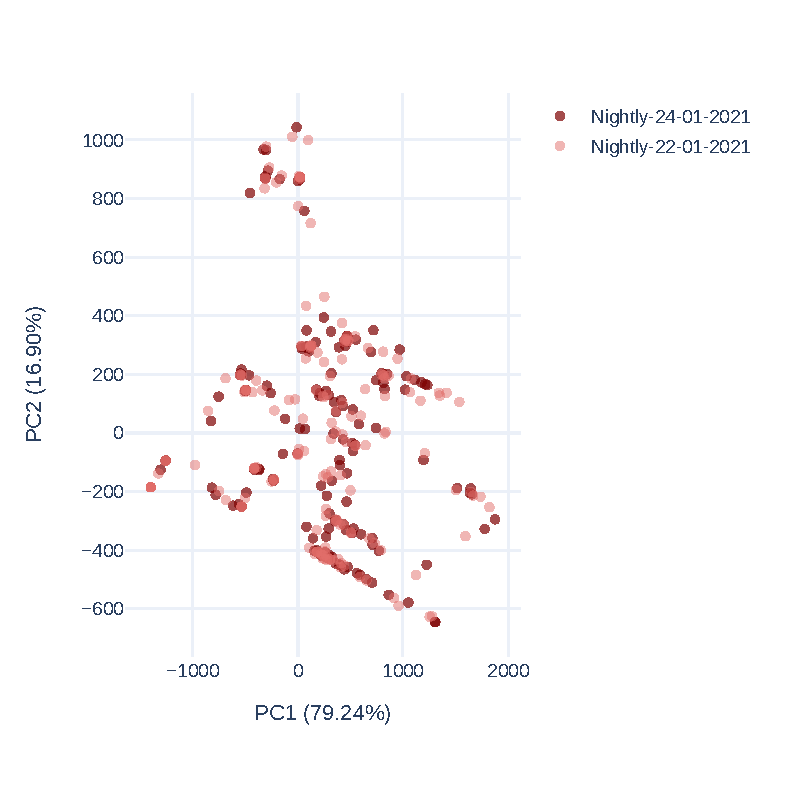
\includegraphics[width=5.52cm]{img/pca-nights-comparison.pdf}}}%
    \qquad
    \subfloat[\centering t-SNE]{{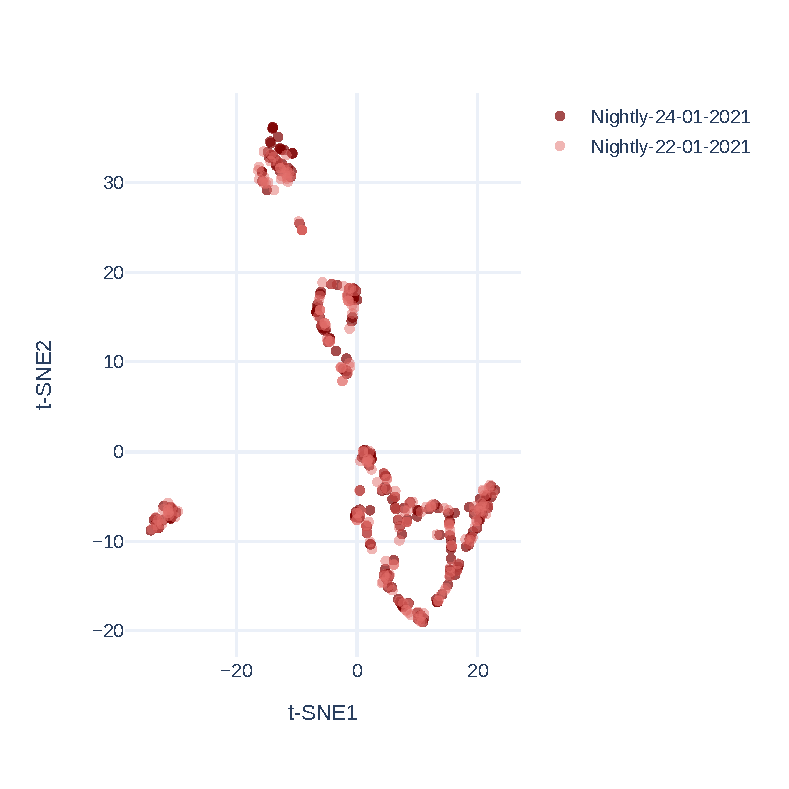
\includegraphics[width=5.52cm]{img/tsne-nights-comparison.pdf}}}%
    \caption{Comparing data from nightly testing obtained from two different dates.}%
    \label{fig:tsne-nights-comparison}%
\end{figure}


\subsection{Calls Group Into A Cluster}
\label{assumption-calls}
In the t-SNE of the Nightly dataset, we could see a cluster of points that we assumed were calls between two radios. The assumption stemmed from the fact that we selected several random data points (log sequences) from this cluster and manually checked the histogram of log templates within the log sequences. It turned out that the vast majority of them represented calls. We will now prove that the observed clustering of points is a cluster of call logs and not an unknown anomaly. We will prove this assumption by highlighting the purpose-built dataset Glostrup Calling in the t-SNE embedding of the Nightly dataset as a central clue to where the call data points cluster.

Figure \ref{fig:tsne-nightly-calls} shows the execution of t-SNE on the scenario described above. After applying feature extraction in $2$ minute windows on the simulated $8$ minutes of calls, we obtain $4$ data points (highlighted by green color). The visualization of the plot indicates that the call data points fall very close to the observed cluster and, moreover, all call data points are consistently close to each other. 

Therefore, we believe that it is possible to determine the class of a clustered set of data points even without using the actual labels. This confirms our assumption that the data from the Nightly dataset is free of anomalies and that the observed cluster is indeed a cluster of calls.

\begin{figure}[h]
    \centering
    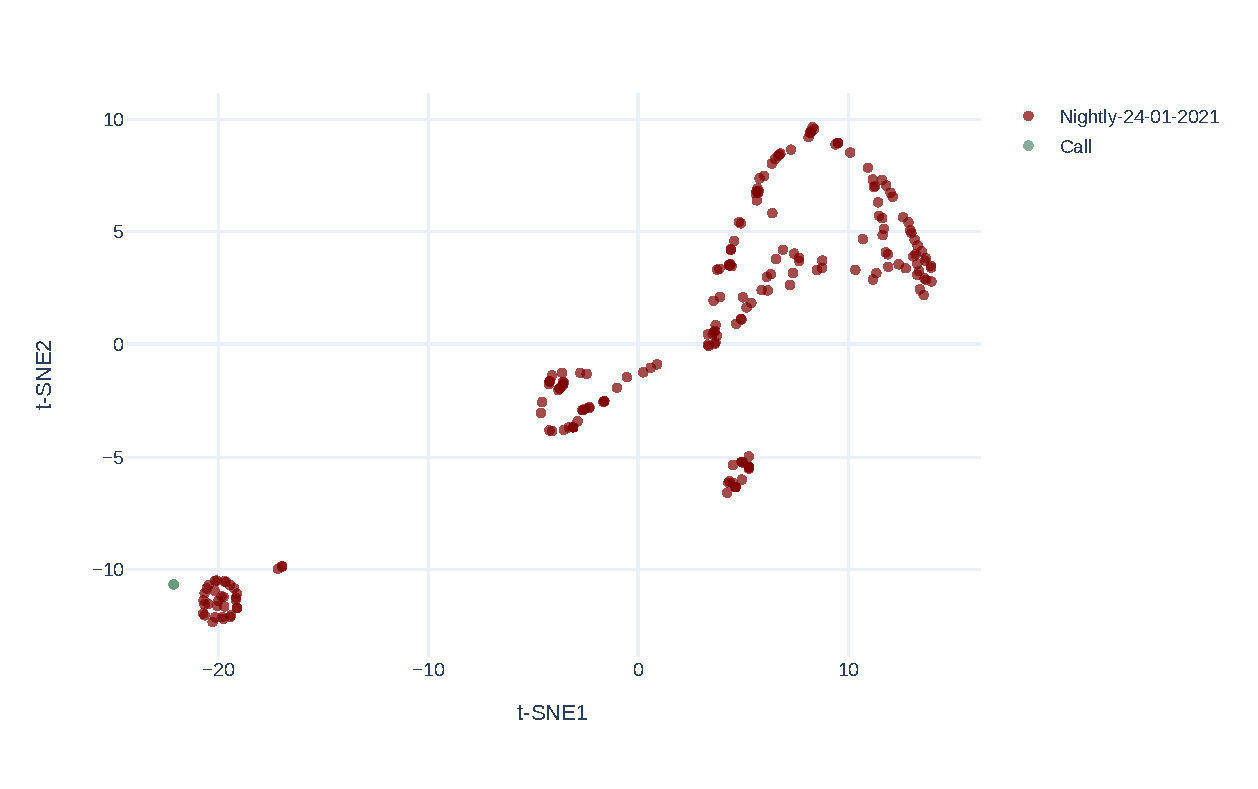
\includegraphics[width=\textwidth]{img/tsne-nights-call-comparison.pdf}
    \caption{Application of t-SNE to the Nightly and Glostrup Calling dataset.}
    \label{fig:tsne-nightly-calls}
\end{figure}

\subsection{Anomalies Are Separable from Normal Data}
\label{assumption-anomalies}
The last assumption we want to check before using the data to train the actual machine learning models, and by far the most important, is to see if anomalies have a tendency to cluster in different regions than normal data. This is crucial because if the human eye can detect an anomaly by looking at a plot, then we can assume that anomaly detection algorithms will also be able to detect these anomalies. 

To prove this, we will plot our Anomalies dataset generated by collecting anomalies during the simulation of the anomaly scenarios described in Section \ref{anomaly_types}. In the PCA and t-SNE plots in Figure \ref{fig:pca-anomalies} and \ref{fig:tsne-anomalies}, the anomaly of Killing Redis is represented by green color and Killing RabbitMQ is represented by blue color. Anomalous data points are plotted with respect to normal points, which are highlighted in red. 

Both plots give us a clear picture that the data points are divided into different clouds of the same anomaly types. Moreover, the anomalous points are outside the normal range. We consider the fact that different anomalies can be successfully distinguished as clusters in the embedding space as an answer to the \textbf{RQ1}. In this case, it is clear that t-SNE gives us a better clustering result than PCA with less points overlapping each other, although both techniques are able to separate the data points into different classes. However, it is interesting to see in the PCA plot, that the Killing Redis anomaly is much closer to the cluster of normal points than Killing RabbitMQ (as mentioned earlier, we should not consider the distances between clusters in t-SNE graphs unless we tune its parameters, so we focus on the PCA graph for cluster proximity analysis). This can be explained as a failure of all brokers in the distributed architecture of the system, which relies on message passing between microservices, causing a major disruption to the entire infrastructure. 
While the malfunctioning Redis cache is an issue that can be fixed relatively easily, the latter causes a severe problem in the application that propagates to many places. Also, as we observed, the broken broker scenario causes the system to be down for a much longer period of time, which gives the services a longer window to generate a larger amount of logs indicating problems.

We obtained a solid indication that feature embedding is informative enough to identify anomaly clusters. We will attempt to further prove this assumption using machine learning.

\begin{figure}[!h]
    \centering
    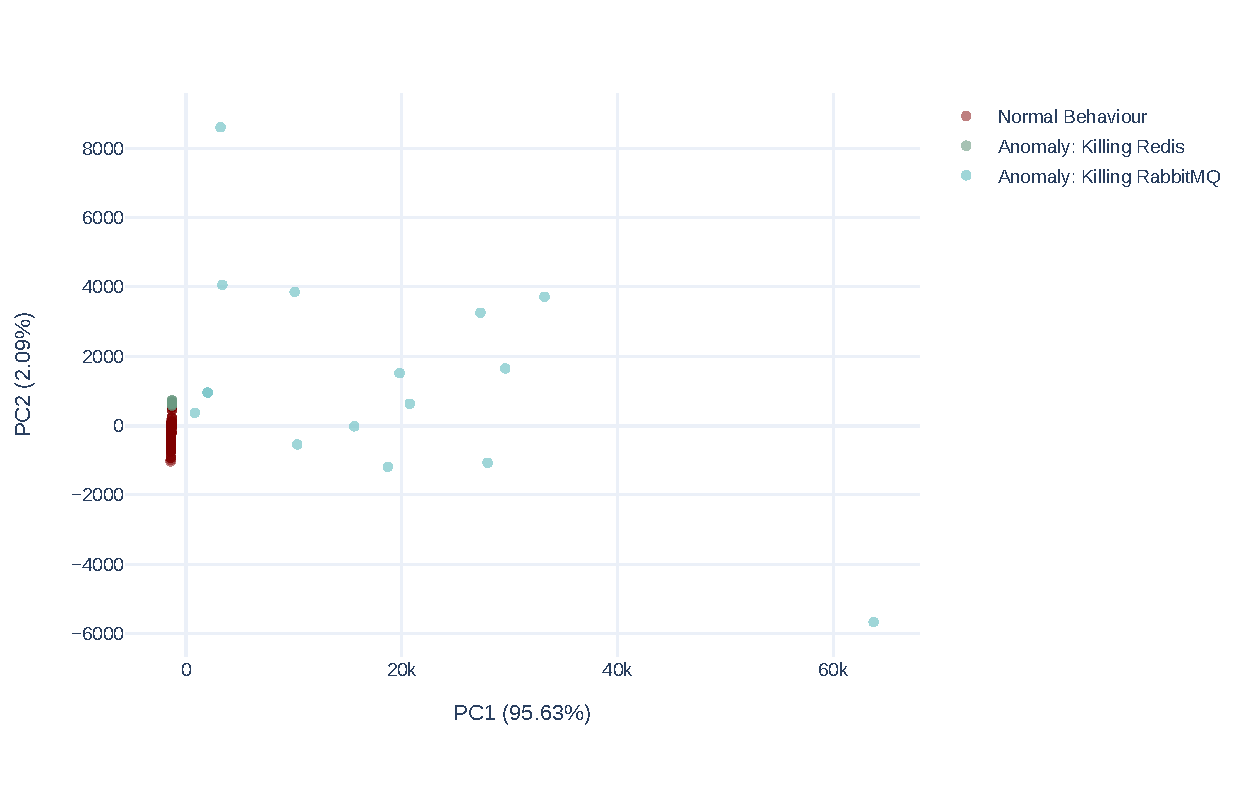
\includegraphics[width=\textwidth]{img/pca-anomalies-vs-normal.pdf}
    \caption{Application of PCA to the anomaly data.}
    \label{fig:pca-anomalies}
\end{figure}

\begin{figure}[!h]
    \centering
    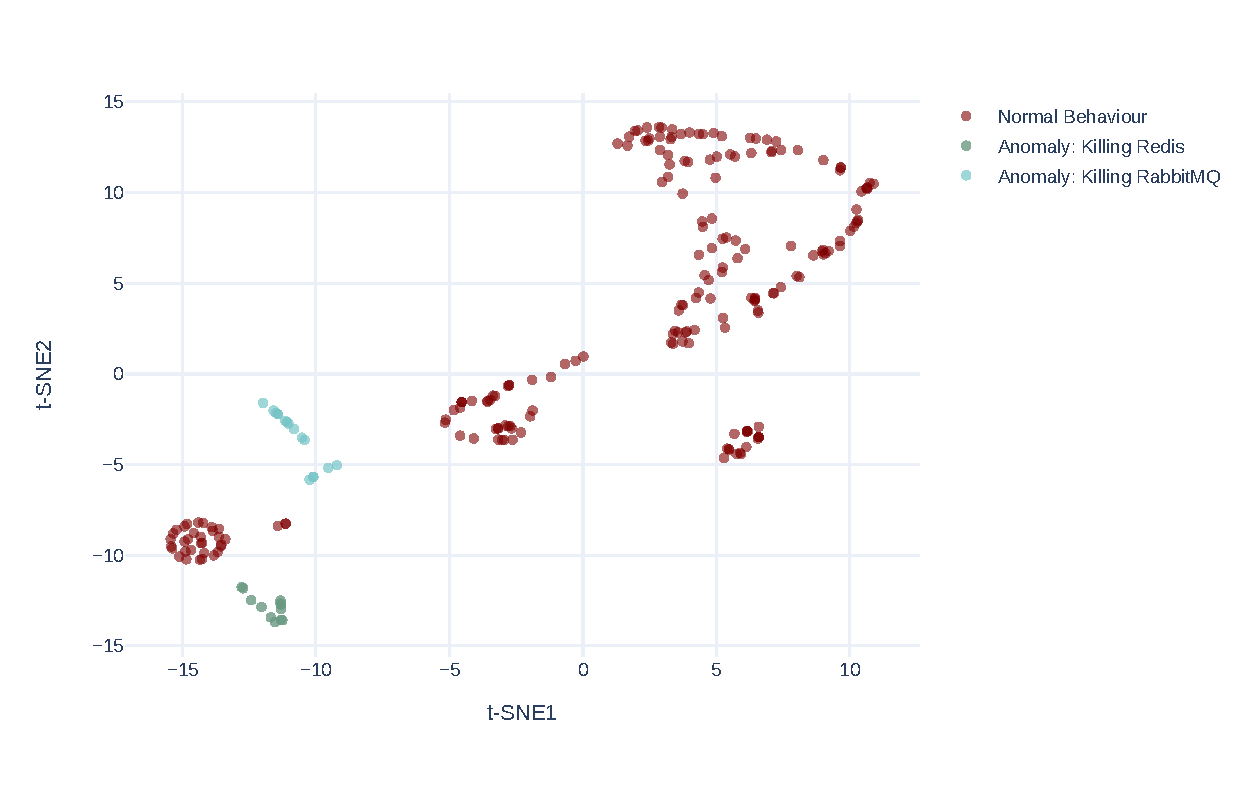
\includegraphics[width=\textwidth]{img/tsne-anomalies-vs-normal.pdf}
    \caption{Application of t-SNE to the anomaly data.}
    \label{fig:tsne-anomalies}
\end{figure}

\section{Evaluation Metrics}
\label{section:evaluationMetrics}
Evaluation metrics are needed to adequately compare different anomaly detection algorithms and different experiment settings.

Let us first introduce four basic metrics: true positive (TP), false positive (FP), true negative (TN), and false negative (FN). ). 

To give an example, let us consider an experimental setting: In a classification task, for each data sample, we assigned a binary label $l$ with values in a set of classes. It is important to note that a class that is normally positive is of particular interest for which the evaluation measure is valid. It gives an information about the correctness of the example in the task of anomaly detection. Moreover, an anomaly detector makes a prediction $\hat{l}$, assigning for each data example whether it classifies it as an anomaly or as a normal data instance. The pairwise relationship of the four counts is explained by the confusion matrix in Table \ref{table:confusionMatrix}. The confusion matrix is a form of contingency table that provides an interpretation of the classifier's performance on a labeled dataset. It is a $2 \times 2$ matrix (in the case of only two classes, but can easily be extended for multiple classes), where the rows represent the actual value of a variable, while the columns represent the predicted value of a variable.

\begin{table}[!h]
\centering
\begin{tabular}{cccc}
\multicolumn{1}{r}{}                 &                              & \textbf{Predicted}          &   $\hat{l}$                          \\ \cline{3-4} 
                                     & \multicolumn{1}{l|}{}        & \multicolumn{1}{l|}{Anomaly} & \multicolumn{1}{l|}{Normal} \\ \cline{2-4} 
                                      
\multicolumn{1}{l|}{\textbf{Actual}} & \multicolumn{1}{l|}{Anomaly}  & \multicolumn{1}{l|}{\textcolor{customBlue}{\textbf{TP}}}     & \multicolumn{1}{l|}{\textcolor{customRed}{\textbf{FN}}}      \\ \cline{2-4} 
\multicolumn{1}{c|}{\textit{l}}                & \multicolumn{1}{c|}{Normal} & \multicolumn{1}{l|}{\textcolor{customDarkRed}{\textbf{FP}}}     & \multicolumn{1}{l|}{\textcolor{customGreen}{\textbf{TN}}}     \\ \cline{2-4} 
\end{tabular}
\caption{An example of a confusion matrix for binary classification.}
\label{table:confusionMatrix}
\end{table}
 
Many meaningful measures can be extracted from the confusion matrix. The evaluation measures are computed on the positive class that is assumed to represent the presence of an anomaly.

\textit{Accuracy} is the most general metric for measuring performance. It simply measures the proportion of correct predictions from all available data points. Accuracy in binary classification is calculated as shown in the following equation:

\begin{align}
    Accuracy = \dfrac{TP + TN}{TP + TN + FP + FN}
\end{align}

However, accuracy alone does not exactly reflect the actual performance of a system designed to correctly detect anomalies. It does not distinguish between the number of correct predictions of different classes \cite{performanceEvaluation2006}. The reason why the accuracy measure is not sufficient in the majority of ML applications is explained later in this section. 

The most commonly used metrics for performance evaluation in machine learning are \textit{precision, recall} and ${F_{\beta}-measure}$. They measure the correct prediction of anomalies within different classes. In our research, we will also focus mainly on these three performance measures.

In order to use them, the problem for which we want to estimate performance must be a classification problem. We assume that our dataset represents a normal behaviour of the system, so that an anomaly detection problem can be translated into a one-class classification problem. 

Precision, recall, and $F_{\beta}$-measure are based on the ratios of counts TP, FP, TN, and FN. 

Precision represents the proportion of correctly detected anomalies out of the total number of anomalies reported. Recall measures the proportion of correctly detected anomalies out of the total number of anomalous data points in the dataset. Finally, the $F_{\beta}$-measure combines these two measures into a single measure. The $F_{\beta}$-measure represents the harmonic mean of precision and recall. If precision and recall are evenly balanced, then $\beta = 1$ and we call it F1-measure. When $\beta > 1$, the score is in favor of precision. On the other hand, it is in favor of recall if $\beta < 1$. 

Let's look at the mathematical formulas for calculating the evaluation measures:

\begin{align}
    Precision &= \dfrac{TP}{TP + FP} \\
    Recall &= \dfrac{TP}{TP + FN} \\
    F_{\beta}-measure &= (\beta^2 + 1) \cdot \dfrac{Precision \times Recall}{\beta^2 \cdot Precision + Recall} 
\end{align}

The reason for the $F_{\beta}$ score is that improving either precision or recall is a trivial task in itself, but the goal is to optimize both simultaneously. The precision metric is more useful when true positives and true negatives are more important. However, false positives and false negatives are considered crucial in most classification problems. Therefore, in these cases, the $F_{\beta}$ score is a better evaluation metric. False negatives and false positives are given more weight, while a large number of true negatives may not affect the score.

Moreover, since anomalies occur much less frequently than normal data samples, we can easily achieve high accuracy without detecting anomalies. For this reason, even though we will be stating the accuracy metric in the result, we will not use accuracy metrics for actual evaluation in this paper.

\section{Experimental Setup}
\label{section:experimental-setup}
In Chapter \ref{chapter:literatureReview}, we described four anomaly detection algorithms: Isolation Forest (\ref{section:lrIsolationForest}), PCA (\ref{section:lrPCA}), Invariant Mining (\ref{section:lrInvariantMining}) and Log Clustering (\ref{section:lrLogClustering}). These algorithms are used to perform the unsupervised anomaly detection experiments. In this section, we will describe the data used in these experiments and discuss the choice of different parameters for each of the anomaly detection methods. To tune the parameters, we will use the evaluation metrics described in the previous section.

\subsection{Dataset}
The dataset used for training the models is the Nightly dataset with data instances of the normal class, hence we also refer to this type of learning as one-class learning. Before training, we start preprocessing the data into numerical vector embeddings in all our experiments indistinguishably according to the methods described in Chapter \ref{methodology}. In Table \ref{tab:training} we give an overview of the statistics related to the dataset used for training and testing.

We used the sliding window technique to divide the dataset into log sequences. The number of resulting sequences depends on the size of the window and a step size. The window size should be chosen to contain the maximum amount of information. We have found that the anomalies we observe in the experiments span at most two minutes. Therefore, we set the window size to two minutes and the step size also to two minutes so that no two windows overlap. As a result, we obtained $201$ log sequences extracted from the Nightly dataset. Each log sequence can be one of two different vector representations: \textit{event count}-vectors and \textit{TF-IDF}-weighted vectors. Therefore, each experiment is run twice with both embedding types.

The length of a vector is given by the number of unique event templates extracted during preprocessing of all datasets used in our research and stored in the state of our log template miner. Thus, at the time of model training, both the number of event types and the length of each log sequence is equal to $3\,963$.

\begin{table}[h]
\centering
\resizebox{\textwidth}{!}{\begin{tabular}{@{}ccccc@{}}
\toprule
\textbf{Dataset} & \textbf{Window size} & \textbf{\# Log sequences} & \textbf{\# Event types} & \textbf{Ratio of anomalies} \\ \midrule
Nightly          & 2 minutes            & 201                       & 3693                    & 0                           \\
Testing          & 2 minutes            & 131                       & 3693                    & 0.22                        \\ \bottomrule
\end{tabular}}
    \caption{Summary of statistics from the Nightly dataset used for training and the Testing dataset used for model evaluation and hyperparameter tuning.}
    \label{tab:training}
\end{table}

\subsection{Software}
To develop scripts for data preprocessing and to run our experiments, Python 3.6.9 was used as the primary programming language. In addition, we used the following Python libraries: 

\begin{itemize}
    \item pandas 1.1.3
    \item numpy 1.19.2
    \item torch 1.7.1
    \item plotly 4.12.0
    \item matplotlib 3.3.2
    \item jupyterlab 2.2.8
\end{itemize}

Exploratory analysis, plotting of data, and preparation of scripts for the ML pipeline are performed using Jupyter Notebook with a Jupyter Lab file browsing interface. Jupyter Notebook is a web-based interactive computational environment for writing Python code that works in a web-based environment. The biggest advantage of using Jupyter Notebook instead of writing Python scripts directly is the ability to run inline code and see the result directly below. It is also possible to add formatted text that improves readability and the reasoning behind the analysis steps.

\subsection{Hardware}
All experiments were performed on a HP ZBook computer with the following technical specification:
\begin{itemize}
    \item Operating System: Linux Mint 19.3 Cinnamon
    \item CPU: Intel Core i7-8850H
    \item RAM Size: 32 GB
    \item CPU Frequency: 2.60 GHz
    \item Internal Storage: 500 GB
\end{itemize}

\subsection{Algorithm Hyperparameters}
Hyperparameters are the values of parameters used to configure a machine learning model, and they must be set before the learning process, which is the main difference from parameters found \textit{during} the learning process. Since the performance of the model is unknown for a given combination of dataset and hyperparameters, it is necessary to explore the range of possible values to obtain optimal hyperparameters. This optimization process is called \textit{tuning}.

The strategy we follow to find optimal parameters is a simple grid search: For each combination of hyperparameter values, we train a model and look at the evaluation metrics for comparison.

Below is a list of hyperparameters and their definitions for all algorithms. The list of values for which they are tested can be seen in Table \ref{tab:hyperparameters}.



\subsubsection*{Isolation Forest}
\begin{enumerate}
    \item \textbf{Number of estimators}: The number of isolation trees generated in the isolation forest, also called the number of base estimators in the ensemble.
    \item \textbf{Max samples}: The number of samples drawn from the input matrix for training each of the iTrees. This number cannot be higher than the number of samples in the input dataset. 
    \item \textbf{Contamination}: Percentage of points in the datasets that are anomalous. The value of the contamination parameter is used during fitting when defining the threshold for the decision function.
    \item \textbf{Max features}: This parameter enables us to control the number of features to pull from the dataset to train each of the iTrees. The maximum value is the number of features in the dataset. 
\end{enumerate}

\subsubsection*{PCA}
\begin{enumerate} 
\item \textbf{Number of components}: Number of output features (principal components) to be extracted in the PCA. If a decimal number is specified, it is used to represent the variance ratio as the principal components 
\item \textbf{Threshold}: The threshold for anomaly detection, which is a value between $0$ and $1$. When this value is exceeded, the sample is considered an anomaly. The threshold value can be set to be automatically calculated using the Q-statistics using the value of the alpha hyperparameter 
\item \textbf{Alpha}: The alpha values for the Q-statistic to calculate the threshold for anomaly detection. 
\end{enumerate}

\subsubsection*{Invariants Mining}
\begin{enumerate}
    \item \textbf{Percentage}: The support ratio, or the percentage of samples that do not break the invariant. We say that an invariant $v_i$ is not broken if the condition $|X_j v_i| < \epsilon $ is satisfied, where $X_i$ is $i$-th sample in the dataset and $\epsilon$ is another user defined parameter. 
    \item \textbf{Epsilon}: A threshold for estimating the invariant space.
\end{enumerate}

\subsubsection*{Log Clustering}
\begin{enumerate}
    \item \textbf{Max distance}: A value of the distance between the clusters, that is used as a threshold to terminate the clustering process. 
    \item \textbf{Anomaly threshold}: The threshold value for anomaly detection scores, which is a distance to cluster anomalies. If this value is exceeded, the sample is considered an anomaly.
    
\begin{table}[h]
\centering
\begin{tabular}{@{}ccc@{}}
\toprule
\textbf{Algorithm} & \textbf{Hyperparameter}                                                                                            & \textbf{Values}                                                                                       \\ \midrule
\textcolor{customGreen}{\textbf{Isolation Forest}}   & \textit{\begin{tabular}[c]{@{}c@{}}Number of estimators\\ Max samples\\ Contamination\\ Max features\end{tabular}} & \begin{tabular}[c]{@{}c@{}}50, 100, 150, 201\\ 150, 180, 201\\ 0, 0.02, 0.03, 0.1\\ 3693\end{tabular} \\ \midrule
\textcolor{customGreen}{\textbf{PCA}}               & \textit{\begin{tabular}[c]{@{}c@{}}Number of components\\ Threshold\\ Alpha\end{tabular}}                          & \begin{tabular}[c]{@{}c@{}}0.85, 0.90, 0.95\\ auto\\ 0.0001, 0.001, 0.005, 0.01\end{tabular}          \\ \midrule
\textcolor{customGreen}{\textbf{Invariant Mining}}   & \textit{\begin{tabular}[c]{@{}c@{}}Percentage\\ Epsilon\end{tabular}}                                              & \begin{tabular}[c]{@{}c@{}}0.98\\ 0.5\end{tabular}                                                    \\ \midrule
\textcolor{customGreen}{\textbf{Log Clustering}}     & \textit{\begin{tabular}[c]{@{}c@{}}Max distance\\ Anomaly threshold\end{tabular}}                                  & \begin{tabular}[c]{@{}c@{}}0.3, 0.5\\ 0.3, 0.5\end{tabular}                                 \\ \bottomrule
\end{tabular}
 \caption{Hyperparameters to be tuned and their respective values which are tested for each anomaly detection method.}
    \label{tab:hyperparameters}
\end{table}
\end{enumerate}

To obtain the optimal hyperparameters, we will run algorithms for each combination of hyperparameters described in the tables above. We will perform these tests using only the basic event count embeddings, and after finding the optimal parameters, we will use them to train the models on the TF-IDF embeddings as well. . 

We evaluate the results of the experiments using the metrics defined in Section \ref{section:evaluationMetrics} to find the optimal hyperparameter values. Since the F1-score combines both precision and recall measures, we select the final set of hyperparameters by the highest F1 score, so we optimize both metrics by optimizing F1. The evaluation is performed on the test dataset. 

It is important to note here that we did not perform any tuning of the hyperparameters of the Invariant Mining model and performed the experiments using the default values set by the Loglizer library. The reason for this is that the process of invariant mining is extremely time consuming and inefficient compared to the other algorithms. It took several hours to train the invariants mining model, while other algorithms were trained in a few seconds. Moreover, we obtained satisfactory results with other algorithms, thereby we decided not to explore further hyperparameter combinations to tune the invariants mining model.

A detailed list of the results of the hyperparameter tuning experiments can be found in the Appendix \ref{appendix:hyperparameterTuning}. A summary of the tuned and final values of the hyperparameters of the specified machine learning approaches used for anomaly detection is given in Table \ref{tab:tunedHyperparameters}. 

\begin{table}[h]
\centering
\begin{tabular}{@{}ccc@{}}
\toprule
\textbf{Algorithm} & \textbf{Hyperparameter}                                                                                            & \textbf{Value}                                                 \\ \midrule
\textcolor{customGreen}{\textbf{Isolation Forest}}   & \textit{\begin{tabular}[c]{@{}c@{}}Number of estimators\\ Max samples\\ Contamination\\ Max features\end{tabular}} & \begin{tabular}[c]{@{}c@{}}100\\ 150\\ 0.1\\ 3693\end{tabular} \\ \midrule
\textcolor{customGreen}{\textbf{PCA}}                & \textit{\begin{tabular}[c]{@{}c@{}}Number of components\\ Threshold\\ Alpha\end{tabular}}                          & \begin{tabular}[c]{@{}c@{}}0.95\\ auto\\ 0.005\end{tabular}    \\ \midrule
\textcolor{customGreen}{\textbf{Invariant Mining}}   & \textit{\begin{tabular}[c]{@{}c@{}}Percentage\\ Epsilon\end{tabular}}                                              & \begin{tabular}[c]{@{}c@{}}0.98\\ 5\end{tabular}               \\ \midrule
\textcolor{customGreen}{\textbf{Log Clustering}}     & \textit{\begin{tabular}[c]{@{}c@{}}Max distance\\ Anomaly threshold\end{tabular}}                                  & \begin{tabular}[c]{@{}c@{}}0.3\\ 0.3\end{tabular}              \\ \bottomrule
\end{tabular}
 \caption{Final hyperparameter values for each anomaly detection method, that are further used for experiments}
    \label{tab:tunedHyperparameters}
\end{table}